\documentclass[onecolumn,10pt]{jhwhw}

\usepackage{epsfig} %% for loading postscript figures
\usepackage{amsmath}
\usepackage{graphicx}
\usepackage{grffile}
\usepackage{pdfpages}
\usepackage{algpseudocode}
\usepackage{wrapfig}
\usepackage{pgfplots}
\usepackage{amsfonts}
\usepackage{booktabs}
\usepackage{siunitx}
\usepackage{commath}

% Default fixed font does not support bold face
\DeclareFixedFont{\ttb}{T1}{txtt}{bx}{n}{12} % for bold
\DeclareFixedFont{\ttm}{T1}{txtt}{m}{n}{12}  % for normal

% Custom colors
\usepackage{color}
\usepackage{listings}
\usepackage{framed}
\usepackage{caption}
\usepackage{bm}
\captionsetup[lstlisting]{font={small,tt}}

\definecolor{mygreen}{rgb}{0,0.6,0}
\definecolor{mygray}{rgb}{0.5,0.5,0.5}
\definecolor{mymauve}{rgb}{0.58,0,0.82}

\lstset{ %
  backgroundcolor=\color{white},   % choose the background color; you must add \usepackage{color} or \usepackage{xcolor}
  basicstyle=\ttfamily\footnotesize, % the size of the fonts that are used for the code
  breakatwhitespace=false,         % sets if automatic breaks should only happen at whitespace
  breaklines=true,                 % sets automatic line breaking
  captionpos=b,                    % sets the caption-position to bottom
  commentstyle=\color{mygreen},    % comment style
  deletekeywords={...},            % if you want to delete keywords from the given language
  escapeinside={\%*}{*)},          % if you want to add LaTeX within your code
  extendedchars=true,              % lets you use non-ASCII characters; for 8-bits encodings only, does not work with UTF-8
  frame=single,                    % adds a frame around the code
  keepspaces=true,                 % keeps spaces in text, useful for keeping indentation of code (possibly needs columns=flexible)
  columns=flexible,
  keywordstyle=\color{blue},       % keyword style
  language=R,                 % the language of the code
  % language=Python,                 % the language of the code
  morekeywords={*,...},            % if you want to add more keywords to the set
  numbers=left,                    % where to put the line-numbers; possible values are (none, left, right)
  numbersep=5pt,                   % how far the line-numbers are from the code
  numberstyle=\tiny\color{mygray}, % the style that is used for the line-numbers
  rulecolor=\color{black},         % if not set, the frame-color may be changed on line-breaks within not-black text (e.g. comments (green here))
  showspaces=false,                % show spaces everywhere adding particular underscores; it overrides 'showstringspaces'
  showstringspaces=false,          % underline spaces within strings only
  showtabs=false,                  % show tabs within strings adding particular underscores
  stepnumber=1,                    % the step between two line-numbers. If it's 1, each line will be numbered
  stringstyle=\color{mymauve},     % string literal style
  tabsize=4,                       % sets default tabsize to 2 spaces
}

\author{John Karasinski}
\title{Homework \# 7}

\begin{document}
%\maketitle

\problem{}
(30 points) Imagine that you are interested in the relationship between mood and weather. You ask 4 people to fill out a questionnaire about their mood for 70 consecutive days and also record the maximum temperature of each day. The data for the weather and the mood from the 4 individuals are in the “tempmood.csv” data set.\\
\\
(a) Plot the data in a way/s that you find meaningful to examine the relationship between mood and weather. Interpret the graph/s.\\
\\
(b) Compute means and standard deviations for the data.\\
\\
(c) Estimate the covariance between weather and mood as well as the sum of cross-products. What does each of these indices indicate about the relation between weather and mood?\\
\\
(d) What is the correlation between weather and mood across all participants? What does the correlation indicate about the relationship between weather and mood?\\
\\
(e) Estimate the regression equation of the line that best represents the relationship between weather and mood for all individuals as a single group.\\
\\
(f) Estimate the regression equation of the line that best represents the relationship between weather and mood for each individual.\\
\\
(g) Test whether the relation between temperature and mood is significantly different between persons using Fisher’s z transformations and z-test.\\
\\
(h) What can you say about differences in the relationship between weather and mood across individuals?\\
\\
(h) You submit the result of all these analyses for publication but the editor rejects the manuscript on the basis of: (i) a lack of power to examine your research questions, and (ii) the fact that there are only 4 individuals in your data and, thus – they claim – you cannot generalize to the population. Nevertheless, you are convinced – or just have a hunch – that there might be something valuable here and write back arguing that the data and analyses are worth disseminating. What would you say to support your argument?\\

\problem{}
(10 points) The following matrices RV and CV are a correlation and a covariance matrix, respectively, of variables $X_1$, $X_2$, $X_3$, $X_4$, and $X_5$. Using the information provided in the matrices, fill in the gray boxes with the appropriate values. Make a note of any anomalies you notice (if any).

\begin{table}[h!]
\begin{center}
\begin{tabular}{rr|rrrrr}
\toprule
  & & $X_1$ & $X_2$ & $X_3$ & $X_4$ & $X_5$ \\
\midrule
            & $X_1$ & ?      & -       & -     & -     & -   \\
            & $X_2$ & -0.5   & 0.25    & -     & -     & -   \\
Covariance  & $X_3$ & 1.8    & ?       & ?     & -     & -   \\
            & $X_4$ & -1.08  & -0.135  & -2.43 & 7.29  & -   \\
            & $X_5$ & 17.28  & ?       &  6.48 & 4.374 & ?   \\
\bottomrule
\\
\toprule
  & & $X_1$ & $X_2$ & $X_3$ & $X_4$ & $X_5$ \\
\midrule
            & $X_1$ & ?      & -       & -     & -     & -   \\
            & $X_2$ & -0.5   & ?       & -     & -     & -   \\
Correlation & $X_3$ & ?      & 0.25    & ?     & -     & -   \\
            & $X_4$ & ?      & ?       & -0.3  & ?     & -   \\
            & $X_5$ & ?      & 0.5     & ?     & 0.3   & ?   \\
\bottomrule
\end{tabular}
\end{center}
% \caption{Results of Simple Effects Analysis}
\end{table}

\problem{}
(20 points) Researchers were interested in the role of extracurricular activities (sports: 0 = other extracurricular activities and 1 = participation in sports) and biological sex (female: 0 = male, 1 = female) on standard normal adolescent perceptions of social acceptance (PSA).

The data can be found in the “socialacceptance.csv” file. Determine whether factors of extracurricular activity type and biological sex are associated with adolescent PSA.\\
\\
a) State the type of design of the study.\\
\\
b) Thoroughly analyze these data for main effects and interactions. Write a report (no longer than a page) in which you report your findings as you would in a journal article (i.e., text, table, and figure).

\problem{}
(10 points) Explain why r must be between -1 and +1. Please, do not use more than 1 or 2 paragraphs. You can append calculations, if you need them.

\problem{}
(20 points) Say you run a simple regression with predictor variable $X_1$ and outcome variable $Y$. You fit the following model:
                $$Y = B_0 + B_1 X_1$$
a) What is the interpretation of $B_0$? What is the interpretation of $B_1$?\\
\\
b) When will $B_1$ be equal to the correlation between $Y$ and $X_1$? Why?\\
\\
After running the analysis you remember a covariate that you believe is related to $Y$, but is not substantively of interest.
c) What are the benefits of including the covariate in the model? Include two benefits and explain them in detail.\\
\\
Finally, you include the covariate within the analysis and fit the following model:
                $$Y = B_0 + B_1 X_1 + B_2 X_2$$
d) What is the interpretation of each of the coefficients in this model?\\
\\
e) When will $B_1$ be equal to the correlation between $Y$ and $X_1$? When will $B_2$ be equal to the correlation between $Y$ and $X_2$? Why?

\problem{}
(10 points) Suppose you are hired to serve as a statistical consultant. In each of the following cases, what advice (if any) would you give to your client concerning the procedures and/or conclusions he or she has drawn, or about the kind of statistical techniques most suitable? Be sure to briefly explain the reasoning underlying your advice.\\
\\
(a) A researcher studies the effects of education (HS or less, Some College, 4 Year College Degree, Graduate/Professional Degree) on income by randomly calling 5,000 participants in the United States. At a presentation of his results several colleagues suggest that effects of education on income may not be robust when considering other predictors such as work experience, time with their current employer, age, personal investments. What sort of analysis did the researcher conduct, and how can the researcher address these criticisms of his research?\\
\\
(b) A researcher is interested in predicting the mental health of college students based on their reported level of stress. What kind of sample should she collect and what statistical technique should she use to achieve this goal?\\
\\
(c) A researcher collected data from undergraduate and graduate students at universities across the country in a study of the relation between age (Range of 18 – 46 years with a Mean = 23.5) and openness. There was a significant, negative relation between age and openness (r(2,998) = -0.13, p < .05). The researcher cited this finding as evidence for why elderly individuals (age 60 years and upward) have difficulty learning about novel technology and ideological shifts; they’re openness has declined substantially over their lives. Is this a reasonable conclusion? Why or why not?\\
\\
(d) A researcher studied a group of 100 students by having them complete a survey once a quarter, every quarter, for two years via an online survey form. The survey consisted of several items meant to measure anxiety, self-competence, and academic performance. What methods of analysis would be applicable to this type of data? How do you justify your recommendations?\\
\\
(e) A researcher received a small grant to conduct a study and is debating on how to spend the money. She is thinking that she can give a test to 300 individuals on one occasion, give a test to one individual on 300 occasions, give a test to 30 individuals on 10 occasions, give a test to 10 individuals on 30 occasions, or any combination of the above. Which of these data collection methods should she use?

\problem{Extra Credit}

(10 points) Explain what it means to say that a correlation is a covariance expressed in z-scores? Derive numerically the formula for a correlation based on the formula from a covariance (and describe the steps in your own words).



% \begin{table}[h!]
% \begin{center}
% \begin{tabular}{l r r r r r}
% \toprule
% Source & $SS$ & $df$ & $F$ & $PR(>F)$ \\
% \midrule
% \it{School Type} & & & & \\
% \hspace{1em} Private     & 29.66 &  2  & 11.97 & $<.001$ \\
% \hspace{1em} Public      & 13.69 &  2  &  5.18 & $ .001$ \\
% \it{Time} & & & & \\
% \hspace{1em} 1      &  0.81 &  1  &  1.1 & $ .295$\\
% \hspace{1em} 2      &  4.00 &  1  &  2.9 & $ .091$\\
% \hspace{1em} 3      & 84.64 &  1  & 44.1 & $<.001$\\
% \bottomrule
% \end{tabular}
% \end{center}
% \caption{Results of Simple Effects Analysis}
% \end{table}

% \begin{lstlisting}[language=Python]
% # Python!
% import pandas as pd
% import seaborn as sns
% sns.set_style('ticks')

% df = pd.read_csv('glong.csv', index_col=0)
% p = sns.lmplot(x='time', y='observation',
%                hue='public',
%                data=df, order=2, ci=95,
%                x_jitter=.3, y_jitter=.3,
%                markers=["o", "x"],
%                legend=False)
% p.axes[0][0].set_xticks([0.5, 1.5, 2.5])
% p.axes[0][0].set_xticklabels(['Sophomore', 'Junior', 'Senior'])
% plt.xlabel('Observation')
% plt.ylabel('End-of-Year Student Confidence Rating')
% plt.savefig('prob5-quad.pdf')
% plt.close('all')
% \end{lstlisting}

% \begin{figure}[h!]
% \begin{center}
% 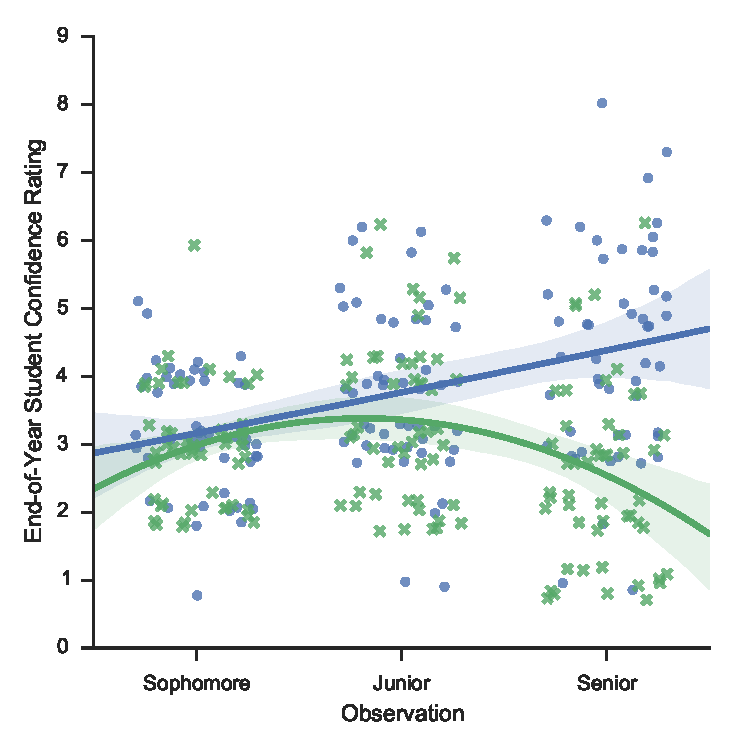
\includegraphics[width=1\textwidth]{prob5-quad.pdf}
% \label{fig:on}
% \end{center}
% \caption{Quadratic trajectories for end-of-year confidence ratings for students in public schools (green) and private schools (blue). Shaded regions represent 95\% confidence regions. (Some jitter introduced for visibility.)}
% \end{figure}


\end{document}
